\documentclass[12pt]{article}

\usepackage{amssymb,amsmath,amsfonts,eurosym,geometry,ulem,graphicx,caption,color,setspace,sectsty,comment,footmisc,caption,natbib,pdflscape,subfigure,array,hyperref}
\usepackage{tikz}
\usepackage{svg}
\usetikzlibrary{arrows.meta, positioning, decorations.pathreplacing}
\usepackage{booktabs}
\usepackage{mathrsfs}
\usepackage{threeparttable}
\usepackage[authordate,backend=biber,natbib,sortcites=true]{biblatex-chicago}
\addbibresource{LiteratureElectric.bib}

\normalem

\onehalfspacing
\newtheorem{theorem}{Theorem}
\newtheorem{corollary}[theorem]{Corollary}
\newtheorem{proposition}{Proposition}
\newenvironment{proof}[1][Proof]{\noindent\textbf{#1.} }{\ \rule{0.5em}{0.5em}}

\newtheorem{hyp}{Hypothesis}
\newtheorem{subhyp}{Hypothesis}[hyp]
\renewcommand{\thesubhyp}{\thehyp\alph{subhyp}}

\newcommand{\red}[1]{{\color{red} #1}}
\newcommand{\blue}[1]{{\color{blue} #1}}

\newcolumntype{L}[1]{>{\raggedright\let\newline\\arraybackslash\hspace{0pt}}m{#1}}
\newcolumntype{C}[1]{>{\centering\let\newline\\arraybackslash\hspace{0pt}}m{#1}}
\newcolumntype{R}[1]{>{\raggedleft\let\newline\\arraybackslash\hspace{0pt}}m{#1}}

\geometry{left=1.0in,right=1.0in,top=1.0in,bottom=1.0in}

\begin{document}

\begin{titlepage}
\title{Investment and the Transfer of Power: Dynamic Effects of Transmission in Electricity Markets\thanks{I thank [PLACEHOLDER: advisors and committee members] for invaluable guidance. I also thank seminar participants at [PLACEHOLDER] for helpful comments. All errors are my own.}}
\author{Dana Golden\thanks{Department of Economics, Stony Brook University. Email: dana.golden@stonybrook.edu}}
\date{\today}
\maketitle
\begin{abstract}
\noindent Renewable resources are essential for energy transition, but their unequal geographic distribution limits adoption in many regions. Long-distance transmission offers a potential solution by connecting renewables-rich areas to high-demand markets. I examine how expanded transmission capacity affects investment decisions by fossil fuel and renewable generators. I develop and estimate a dynamic model of generator behavior consisting of a short-run optimal dispatch problem incorporating line losses and transmission constraints between zones and a long-run dynamic game for capacity investment. Using data from six ISOs in the Eastern Interconnection and ERCOT from 2018--2023, I find that upgrading all inter-zonal transmission to modern HVDC standards would reduce average wholesale prices by 6\%, generating approximately \$4 billion in annual welfare gains---roughly one-third of total congestion costs. Even partial upgrades (50\% of lines) achieve over 5\% price reductions. Regional effects are heterogeneous: the Northeast experiences the largest price declines while the Midwest sees modest increases. In the long run, adding major transmission projects such as the Grain Belt Express increases solar and wind adoption in the Eastern Interconnection by over 10\% by 2050. I use these estimates to evaluate proposed policies including the Big Wires Act, the Inflation Reduction Act, and the Bipartisan Infrastructure Law, finding that transmission investment and renewable subsidies act as complements rather than substitutes in accelerating the energy transition.\\
\vspace{0in}\\
\noindent\textbf{Keywords:} Electricity, Transmission, Capacity Investment, Renewable Energy, Dynamic Games\\
\vspace{0in}\\
\noindent\textbf{JEL Codes:} Q40, L94, Q54, C73\\

\bigskip
\end{abstract}
\setcounter{page}{0}
\thispagestyle{empty}
\end{titlepage}
\pagebreak \newpage




\doublespacing


\section{Introduction} \label{sec:introduction}

Climate change remains the most important environmental issue facing the world at present. In order to prevent catastrophic impacts of climate change, economies need to decrease greenhouse gas emissions. Electricity was associated with the highest share of carbon emissions in the United States, 31 percent in 2022 according to the Energy Information Administration, and has continuously provided the largest source of greenhouse gas emissions for decades \autocite{EIAReport}. Renewable energy provides the clearest pathway to a reduction in electricity-related greenhouse gas emissions. Currently, a major project is underway throughout the developed world and the United States in particular to replace fossil fuel generators with renewable generation.

However, two persistent problems plague the renewable energy transition. First, the unequal dispersion of potential for renewable resources makes renewable generation infeasible in vast swaths of the United States. The climate of states like New York and New Hampshire presents significantly less potential for renewable generation than that of states like Texas and Nevada. Texas and Nevada have abundant sun and wind, which have allowed renewable energy to flourish. The area required by solar and wind also means that the locations with the highest propensity for renewable generation often are further from cities. Second, renewable resources tend to be intermittent. The sun shines only for so many hours a day, and when the wind blows demonstrates marked variability. As electricity must always balance, intermittency can cause instability in electric grids. If too much electricity enters the system at one time, it can cause an overload and lead to system outages. Storage has been proposed as a potential solution for the intermittency problem but remains costly and limited. Storage also does not provide a solution in areas with limited ability to take advantage of any renewable energy.

Increasing transmission, the ability to send electricity between zones, provides another potential solution to the problem of intermittency and dispersion. Time-zone and geographic differences ensure that the peak hours for sunlight in Kansas coincide well with the peak demand hours in Indiana, and increasing long-distance transmission increases market interconnectedness, which decreases risks of instability and renewable energy curtailment, the forced shutdown of renewable resources due to over-supply. While long-distance transmission has previously proved largely infeasible both technically and economically, advancement in technologies such as High-Voltage Direct Current (HVDC) and High-Voltage Alternating Current (HVAC) provide a method through which to increase the range of transmission and potentially facilitate greater connection of renewables to the grid. Similarly, the transition from fossil fuel resources that could be easily transported to renewable resources increases economic viability of transmission expansion. Despite its potential merits as a technique to increase adoption rates for renewable energies, transmission expansion has largely escaped examination by economists.

%How do utilities choose which lines to invest in when it comes to long-range transmission, and 
How does long-run investment in transmission impact capacity investment in renewable resources? At face value, the direction of the welfare effects of transmission expansion may seem trivially positive as is the case in most problems of friction reduction; however, because of the substantial cost of increasing transmission capacity combined with the dynamic effects of firm investment, the sign of welfare change remains ambiguous without further study. Increasing transmission tends to lead to equilibration of prices across markets and thus may lead lower prices to cause exit in some markets and higher prices to cause entrance in others. Exiting firms may cause blackout and decreased reliability, which can cause significant losses in consumer welfare due to the high inelasticity of the demand curve for electricity. Beyond first order welfare and reliability effects, emissions produced must be examined. 

Two main counterfactual experiments are performed to examine policy impacts. First, the impacts of the increased subsidization of investment in long-range transmission infrastructure are examined through the lens of the Bipartisan Infrastructure Law. This enters the model through changes in the adjacency matrix representing the ability to send electricity between locations. Second, the impacts of subsidization in renewable energy technology through the Inflation Reduction Act are examined. By performing the experiments separately and together, it can be determined if subsidization of transmission infrastructure is an alternative to subsidization of renewable generation or simultaneous subsidization policies complement each other.

Recent work within the industrial organization literature has taken a profound interest in the determinants of long-run investment in the electricity market as it relates to energy transition. \cite{butters2021soaking} examine the issue of battery investment to reduce intermittency as it relates to the California Independent System Operator (CAISO) market while \cite{elliott2022investment} uses an oligopolistic model to consider the potential impacts of carbon taxes and capacity payments on the resource mix in Western Australia. While both consider the dynamics of the electricity market, both also assume that prices are constant throughout the entire region and cannot be used to analyze locations with more than one settlement point.  More recent work by \cite{gowrisankaran2024energy} connects changes in the price differential between natural gas and coal to widespread changes in capacity investment away from coal to natural gas. \cite{arkolakis2023clean} integrates the impacts of transmission into a macro model and considers how the implementation of proposed projects might impact further adoption of renewable energy. Though Arkolakis and Walsh's work considers a similar question, the question is approached from a macro perspective and so, the dynamics of individual firms are neglected providing an important source of future research the current work addresses. 

\cite{gonzales2022dynamic} considers the implications of interconnection between the Northern and Southern Chilean electricity markets for long-run entry and exit. My work extends their work by generalizing the model to deal with larger and more complex grids. My work also goes further by utilizing variation in spatial transmission capacity to examine transmission's impact without significant temporal variation in transmission infrastructure.

The inclusion of generator investment based on price differentials between locations marks a major contribution to the literature. Real-world limitations on the movement of electricity make ignoring transmission perilous, and the need for investment in renewables makes a valuation of transmission expansion including its effects on renewables investment increasingly pertinent. Consideration of how interconnected electricity markets function together even on short time scales also remains conspicuously absent from the industrial organization literature around electricity providing a gap for research. 
%The model also has potential usage outside of electricity markets as it examines the problem of endogenous network formation, a problem of perpetual interest to microeconomists.

I examine the behavior of generators providing electricity in the wholesale market by building a theoretical model of the short-run electricity market and connecting the model to a dynamic game in the long-run electricity market where generators enter and exit. The model builds on prior work in electricity by adding constrained trade between regions in electricity. I estimate the short-run model using maximum likelihood, and I estimate the long-run model using a fixed-point generalized method of moments methodology, which combines the moment inequality approach for dealing with multiple equilibria from \cite{holmes2011diffusion} and the strategy for estimation capacity investment in dynamic games found in \cite{gowrisankaran2024computable}. I run the counterfactuals by adjusting the available set of long-range transmission lines in the United States and the fixed costs and entrance costs of the generators in line with the legislation considered.
%I follow \cite{holmes2011diffusion} and \cite{pakes2015moment} in estimating the long-run model through the moment inequality method

 The paper is organized as follows. Section \ref{sec:literature} reviews the prior literature related to transmission as well as investment in the electricity market. Section \ref{sec:data} describes the structure of the market analyzed and presents descriptive statistics about the market. Section \ref{sec:Model} presents a structural model, while Section \ref{sec:Estimation} describes the estimation strategy using the structural model. Section \ref{sec:result} provides a description on results and model-fit.  Section \ref{sec:Counterfactuals} details counterfactuals. Section \ref{sec:conclusion} concludes the paper and provides further research directions.

\section{Literature Review} \label{sec:literature}

The literature related to the question of the impact of congestion on investment by generators in the electricity market falls in three distinct categories: discussions of the problems related to a changing resource mix in the electricity market, examinations of investment decisions by firms in the electricity market, and considerations of the impacts of congestion on firm behavior. 

A rich body of literature exists related to the current energy transition the United States and the world is undergoing as it relates to electricity markets and firm behavior in these markets. \cite{gowrisankaran2016intermittency} examines intermittency of renewable resources and how the intermittency impacts the electricity market. \cite{gowrisankaran2016intermittency} finds that intermittency accounts for a substantial portion of social costs related to renewable energy and that intermittency presents a major barrier to a grid powered mainly be renewable energy. More recently, \cite{gowrisankaran2024energy} examines the rationale for utility's shift away from coal and towards natural gas. The paper utilizes an estimation technique popularized by \cite{gowrisankaran2024computable} to understand how the increasing price differential between coal and natural gas led to a shift in the resource mix and substantial changes in capacity investment. My estimation strategy borrows substantially from this strain, especially in the creation of an estimation strategy but utilizes a dynamic game to consider the actions of multiple generation companies together, takes into account the shift towards renewables, and integrates transmission into the model.

Related to the body of work on a changing resource mix comes a substantial group of papers that ask the question of how firms choose to invest in and enter electricity markets. \cite{butters2021soaking} examines the impact of California's battery capacity mandate on battery adoption and electricity markets. The paper builds a model of the operations of battery storage facilities in the day ahead and real time markets and relates the operations model to the long-run market for storage capacity. The paper concludes with a series of implications relating to policy and also the impacts of differing assumptions about depreciation and capital changes over time. The paper finds that the mandate increases social welfare slightly after considering capital costs even before taking into account the impacts on reliability. 

\cite{elliott2022investment} builds on \cite{butters2021soaking} by building a model of investment in generators in the Australian electricity market. Elliot's model divides generation companies into strategic firms whose entry and exit impacts price and fringe firms and then uses this division to model a dynamic game in which firms choose to add or subtract generation from their portfolio in the long-run. Elliot utilizes the model to run a series of counterfactuals with the primary focus on changes to carbon taxes and the capacity market. Both models provide a useful framework to consider the impact of policy on long-run firm behavior in the electricity market.

\cite{holland2022decarbonization} provides the first model from the literature to consider multiple wholesale markets simultaneously. Holland uses EIA data on generation mix and load to model the impacts of several market policies including increasing transmission on renewables adoption and social welfare in the electricity market. While \cite{holland2022decarbonization} proves ambitious, the model considers regional markets as homogeneous and makes the strong assumption that increasing transmission simply means all generators have access to all load. The current work builds on this modelling by considering a more realistic model of transmission and congestion in an electricity market with equilibria determined at the node level.

Finally as the current work examines the impact of transmission on investment, the work focuses heavily on the impacts of transmission on markets and the firms that operate in them. \cite{arkolakis2023clean} builds a macro-style model of the process of growing the economy while also converting to clean energy. Within the model, transmission is considered as well as the impacts of transmission expansion; however, very little consideration is given as to how the energy markets function and the endogenous process of market investment by resources.

\cite{gonzales2022dynamic} performs the most similar research to my work. The paper also has a model of long-run dynamics within the Chile electricity market and estimates the impacts of a grid expansion connecting the Northern and Southern regions of Chile on entry and exit of renewables and fossil fuels. The short-run model used to relate transmission expansion to prices is very simplistic and does not allow for settlement at multiple points simultaneously. It also requires generation data, which are not available for the United States. As the American grid is substantially larger and more complex, the expansion of \cite{gonzales2022dynamic} I perform by adding these features presents a valuable contribution. 

Finally, \cite{gonzales2022dynamic} does not seriously consider the interdependence of generators in its long-run model. My model utilizes a dynamic game for the long-run stage, which allows for a more accurate model of transmission's impact on capacity investment. This is because within a transmission framework, long-run capacity choices are fundamentally interdependent. When considering transmission, the decision to invest in solar in Nebraska impacts the choices of Indiana coal plant owners, making this consideration valuable.

The current work builds heavily on prior work conducted by \cite{butters2021soaking}, \cite{elliott2022investment}, \cite{gonzales2022dynamic}, \cite{gowrisankaran2024energy} related to investments in electricity markets to understand the determinants of investments in increased capacity at the grid level. 

My work expands on prior work by incorporating congestion data from multiple markets simultaneously to examine how increased transmission impacts prices in the real time market and linking this to the dynamics of generation investment in the long-run market. The work advances the field by combining the considerations made by \cite{gonzales2022dynamic} for transmission in short-run electricity markets with a capacity adoption model with a dynamic game similar to the long-run model found in \cite{elliott2022investment}. In estimation, the work takes its inspiration from recent advances in the estimation of capacity games from \cite{gowrisankaran2024computable} and \cite{pakes1998empirical}. Combined, these frameworks allow for a more realistic analysis of transmission's impacts.


\section{Setting and Data} \label{sec:data}

\subsection{Setting}
In most of the United States, the electricity market is divided between the wholesale and retail markets. In wholesale markets, generators sell electricity to utilities who then sell the electricity to end-users in the retail market. Wholesale market prices are generated through the locational marginal price (LMP) mechanism. Generators submit bids of price-quantity pairs that determine how much an individual generator is willing to supply at a series of set prices. The equilibrium price is thus the price at which the last economically dispatched generator bids for the final unit of electricity. This price is paid to all generators that are dispatched at a particular market location.

We focus on the wholesale market for electricity in the Eastern Interconnection and ERCOT. We choose to focus on the regions with wholesale markets because wholesale markets have readily available price data and because vertically integrated retail markets function differently. The focus on the Eastern Interconnection comes from the fact that the majority of US ISOs are in the Eastern Interconnection. The addition of ERCOT provides the ability to perform counterfactuals examining expanded interconnection between ERCOT and the Eastern grid.

\subsection{Dataset Creation}

Data for the short-term model came from EIA form 923, EIA form 860, EIA form 930 data, EPA's Power Markets Data, the individual ISOs, S\&P capital IQ Global, Homeland Infrastructure Foundation Level Database (HIFLD), and Meteostat. The model was estimated on data from 2018 to 2023 at the zonal level. The zonal level was chosen to increase the proportion of binding transmission constraints in the data and to increase granularity of the dataset in terms of both generators and load sources.

From each individual ISO, I took price and load data at the zonal level. I then took hourly fuel mix data at the zonal to estimate generation by generator by hour. For fossil fuel generators covered by CAMPD, the generation by hour was available. However, for other generators, the generation needed to be estimated. In order to estimate generation by hour by generator, EIA Forms 923 and 860 were combined with ISO data on fuel mix. Percentage of generation by the generator was found by taking the percentage of total generation for the zone by month by generation owner from Form 923. The value was then multiplied by the generation for the fuel type for the hour. If generation by the generator was greater than generation capacity, the generation was reduced to the generation capacity, and generation was redistributed to the remaining generators.

In order to estimate transmission capacity and line losses between zones, the HIFLD data on the electricity grid was utilized. The data allowed me to build a full dataset of transmission capacity and line losses in 2022. A line was considered to connect two zones if the line started at a substation in one zone and ended at a substation in another. Using this approach for connection estimation has the downside of neglecting flows that went between multiple substations and zones. However, this works well with the assumption of the grid as a bipartite network from the model. The HIFLD data contained information on type of line, voltage, length, and location. This was used to estimate flow limits and line losses based on engineering assumptions according to the technique discussed in Appendix \ref{sec:appendixc} following \cite{arkolakis2023clean}. To get historical changes in transmission capacity and line losses, I solved for transmission capacity additions and retirements based on S\&P Capital IQ's transmission projects dataset. These were added to the transmission capacity and losses from the HIFLD data to get the transmission capacity from 2001 to 2024.

With the approximate generation data for generators that did not report to the EPA and the exact costs for generators that did report to the EPA, the exports from each zone to each other zone were estimated. To estimate exports, I first added net exports to zones outside of the area of interest. Net exports to outside areas by hour were taken from EIA form 930, which provides data on flows between balancing authorities at an hourly level. Where a balancing authority outside of the dataset connected to multiple zones in the dataset, net exports are added to load proportionately to load in each of the connected regions. 

Given data on load and approximate generation, an optimal dispatch problem was solved for each hour based on the generation by generator, transmission capacity and line losses. Generation was dispatched from zones with low LMP to zones with high LMP in order of marginal cost based on heat rate and fuel cost until all load was satisfied and all generation was distributed. Marginal cost was estimated using fuel cost data from EIA Form 860 and heat rate data from EPA CAMPD data. For resources without marginal cost data from EIA, an order of dispatch was provided by resource type with solar, hydro, geothermal, and wind dispatched first with ties distributed based on capacity size. Nuclear was then distributed followed by fossil fuel resources for which marginal cost data at the monthly level was available. Firms with lower marginal costs per unit of generation were dispatched to regions earlier. I use these export data to estimate hourly marginal cost curves in the short-term model.

The characteristics of the zones impacting marginal cost of the generators were taken from EIA form 860, Meteostat, and S\&P Capital IQ Global. EIA provided information about the generation companies in terms of ownership and characteristics of generators. Meteostat provided data on weather hourly in the zones. In order to get an average weather for the zones, a centroid was taken from each zone. Weather data thus represent the data at the weather station closest to the centroid of the zone.

Data for the long-term model came from EIA Form 860, EIA's Annual Energy Outlook (AEO), NREL's Standard Scenarios, and S\&P Capital IQ Global. The long-term model was estimated on historical data going back to 2001 with forward-looking generators basing capacity decisions on revenues estimated until 2050 after which the fuel mix and load profile are assumed constant and an infinite sum is taken. The year 2050 was chosen because it was the last year of projections from AEO and because it is a date at which most pledges for energy transition are based.

EIA form 860 provided data on capacity of generators between 2001 and 2024. These data were aggregated by owner, zone, and resource type to get capacity for long-term model estimation. For resources of types not modelled such as nuclear and hydroelectric, the capacity was taken from the aggregate capacity by zone. Meteostat and Prism provided historical long-term weather data. S\&P Capital IQ Global and EIA provided data on historical natural gas prices and coal prices.

Most data from the projections for years in the future come from EIA's Annual Energy Outlook (AEO) for 2023 and NREL's Standard Scenarios with Cambium. The AEO has data on projected load by region, projected natural gas and coal price, and projected capacity and generation for nuclear and other generation types. In order to get projections for long-term changes in transmission capacity for the long-term model, NREL's Standard Scenarios were utilized. The Standard Scenarios also provided long-run data on transmission and distribution losses, load growth, and future capacity for fuels not in the model.

The current study will consider data only from Independent System Operators in the Eastern Interconnection and the Electric Reliability Council of Texas (ERCOT). For a map of the zones of interest, refer to Figure \ref{ZoneMap}. This includes the Southwest Power Pool (SPP) which governs parts of the Midwest from Oklahoma to Wyoming. The Eastern Interconnection also includes the Midcontinent Independent System Operator (MISO) which governs the Midwest east of Mississippi to Nebraska as well as Pennsylvania-New Jersey-Maryland Interconnection (PJM), New York Independent System Operator (NYISO), and ISO New England, which governs all states on the Eastern Seaboard North of New York. Outside of the Eastern Interconnection, data are also provisioned from the ERCOT, which includes much of Texas.

\subsection{Descriptive Statistics}

Table \ref{priceData} shows how prices and loads differ between the different Independent system operators. There is significant variation with ISO-NE having the highest mean price and SPP having the lowest. Load also varies by ISO with PJM, the largest ISO also having the highest load. Figures \ref{fig:PriceMap} and \ref{fig:PriceLoad} show how load varies across the sample by zone. Load differs both within a time dimension and across the spatial dimension with peaks in load profiles in differing by time zone and weather conditions and larger more densely populated zones having more load. Table \ref{ShortTermStats1} provides descriptive statistics on the estimated features of the hourly dispatch model including hourly exports by generator and hourly generation by generator type. Table \ref{ShortTermStats2} provides descriptive statistics for the short run characteristics and the variables that feed into the short-run model.

Figure \ref{fig:CapacityFactorbyISO} shows how estimated capacity factor differs by ISO. Capacity factor is the ratio between total generation and total capacity and indicates the efficiency of a particular generator or generators in a particular location.

\section{Model} \label{sec:Model}

\subsection{Short-run Model}

Under certain conditions, the generator problem is identical to the social planner problem. The conditions for equivalency are based on \cite{gilbert2004allocating} and \cite{cramton2017electricity} and include no market power among generators, no gamesmanship or non-competitive bidding, increasing marginal cost curves, and linear constraints. The assumption of increasing marginal cost curves is consistent with bid offer data provided by generators and also economic theory. Gamesmanship and non-competitive bidding are outlawed and highly policed by the Federal Energy Regulatory Commission. The most dangerous assumption is thus the non-existence of market power. As \cite{gilbert2004allocating} notes, transmission constraints can and often do lead to market power; however, due to competitive market pressures and regulations limiting bidding ability, sustained market power in the electricity market proves elusive. Due to the value of the equivalency, the assumptions are made, and the problem is solved as a social planner's problem.

Additionally, I aggregate to the resource and ISO level. This needs to be done in this case because the data do not include generator data by hour and only include generation data at the resource level but is not ideal as it loses a great deal of granularity, which is extremely valuable in a model of transmission. Where data are available, I disaggregate as much as possible. The ISO resource dispatch problem follows.

The ISO solves a static problem each hour where it chooses how much quantity $q_{ijkt}$ to send to each individual demand node from each resource $k$ at each supply node $j$. The ISO minimizes the cost of generation by dispatching less costly resources earlier subject to system constraints. The profit maximization problem is thus equivalent to a cost minimization problem, and the objective function can be written as

\begin{equation}
\pi_{t}=\max_{\{q_{ijkgt}\}_{i,j,k,g,t\in I,J,K,G,T}} [-\sum_{i=1}^I\sum_{j=1}^J \sum_{k=1}^K \sum_{g=1}^G c_{jkgt}(x_{jkgt},q_{ijkgt},\epsilon_{ijkgt})].
\end{equation}

The profit function faces a few constraints that limit potential choices based on the constraints from the generator. First, the combined ISO cannot transmit between two locations more electricity than a line permits;
 
 \begin{equation}
    \sum_{k=1}^K q_{igjkt}\leq A_{ij} \forall i,j,t.
 \end{equation}

\noindent The ISO cannot dispatch more than a resource's maximum capacity $O_{jt}^{MAX}$ at any particular time;
  \begin{equation}
     0\leq \sum_{i} q_{igjkt}\leq O_{jt}^{MAX} \forall j,k,t.
 \end{equation}

This can be written mathematically as the budget constraint;
 
  \begin{equation}\label{Budget_Constraint}
     \sum_{j=1}^J\sum_{k=1}^K (1-B_{ij})q_{igjkt}=L_{it} \forall i.
 \end{equation}

%An equilibrium in the operations model occurs when all generators offer electricity optimally, utilities optimally choose generators to dispatch, and wholesale price is equal to the marginal cost of the last economically dispatched resource such that the market clears.


If no constraints bind, resources set marginal cost equal to price and produce where price is highest. If the lowest cost resource faces the transmission constraint, it will be dispatched for up to $A_{ij}-\sum_{g'\neq g} q_{ig'jkt}$ units of electricity in the location with highest price, then sell up to $A_{ij}$ units of electricity to the location with the second highest price and repeat this process until either maximum generation $O_{jt}^{MAX}$ is reached, or marginal revenue is equal to marginal cost. The prices received by resources are then equal to the marginal cost of the last economically dispatched resource as explained in section 3.1. The full ISO problem can be written as

\begin{equation}
\pi_{t}=\max_{\{q_{ijkgt}\}_{i,j,k,g,t\in I,J,K,G,T}} [-\sum_{i=1}^I\sum_{j=1}^J \sum_{k=1}^K \sum_{g=1}^G c_{jkgt}(x_{jkgt},q_{ijkgt},\epsilon_{ijkgt})] \mspace{18mu} s.t.
 \end{equation}
   \begin{center}
     $\underbrace{\sum_{j=1}^J\sum_{k=1}^K \sum_{g=1}^G (1-B_{ij})q_{ijkgt}=L_{it}}_\text{Resource constraint} \mspace{18mu} \forall i$
 \end{center}
 \begin{center}
    $\underbrace{\sum_{k=1}^k \sum_{g=1}^G q_{ijkgt}\leq A_{ij}}_\text{Transmission constraint} \mspace{18mu} \forall i,j,t$
 \end{center}
   \begin{center}
     $\underbrace{0<\sum_{i} q_{ijkgt}\leq O_{jkgt}^{MAX}}_\text{Capacity constraint} \mspace{18mu} \forall j,k,g,t.$
 \end{center}

 Blackouts are not allowed in the current iteration of the model. This means that, by assumption, there is enough electricity to satisfy all load at every node at any given time. Additionally by assumption, no resource is ever transmission-constrained at all locations. Finally by assumption, within each generation node $j$, at least one resource is not at maximum capacity at any given time.

The method for solving the operations model is detailed in Appendix \ref{sec:appendixa}. The solution is reminiscent of other trade models. The error for a constrained generator should be equal to the difference between the marginal cost of the generator and the marginal cost of the marginal generator combined with the costs of the transmission and capacity constraints where the transmission and capacity constraints can be solved for by comparing the costs for generators at unconstrained nodes with generators at constrained nodes.

\begin{equation}\label{mlequation}
\tilde{V}_{ijkgt}=\underbrace{x_{jkgt}\beta+q_{ijkgt}\nu_k}_\text{MC resource}-\underbrace{\frac{(1-B_{ij})}{(1-B_{ij''})}[LMP_{it}]}_\text{MC marginal resource}
\end{equation}
\begin{center}
$+\underbrace{q_{i'jkgt}\nu_k-q_{ijkgt}\nu_k+\frac{LMP_{i't}}{(1-B_{i'j''})}(1-B_{i'j})-
\frac{LMP_{it}}{(1-B_{ij'''})}(1-B_{ij})}_\text{cost of transmission constraint}$

$+\underbrace{(x_{jk'g't}\beta+q_{ijk'g't}\nu_{k'})-(x_{jkgt}\beta+q_{ijkgt}\nu_k)}_\text{Cost of capacity constraint}$.
\end{center}

\noindent For the generator $jg'k$, 

\begin{equation}\label{cap3}
\tilde{\epsilon}_{igj'kt}=\epsilon_{igjkt}-\epsilon_{i'g'jkt}
\end{equation}

\noindent for any nodes $ijk'$ with transmission constraints but without capacity constraints, and 

\begin{equation}\label{cap2}
\tilde{\epsilon}_{i'jk't}=\epsilon_{i'jk't}
\end{equation}

\noindent for $i'jk'$ neither transmission nor capacity constrained. Each $j$ node has one resource that is not capacity constrained, and each resource has at least one $i$ node with which it is not transmission constrained. Thus, by plugging equation \ref{cap2} into equation \ref{cap3} and Equation \ref{cap3} into Equation \ref{cap1}, we can solve for each $\epsilon_{ijkt}.$

Define $P_t$ to be a multivariate normal probability density function with mean zero and variance $\Omega_1$ at time t from which the errors at time t $\epsilon_{ijkt}$ are drawn. This leads to a likelihood function for each t and each combination of a resource at location $ijk$ except the marginal resource that sets the LMP,

\begin{equation}\label{likelihoodFunction}
L_1= \prod_{t=1}^{t=T} P_t(\tilde{V}_{111t},...,\tilde{V}_{IJKt}).
\end{equation}

\noindent By maximizing this likelihood function, I can estimate $\nu_k$ and $\beta$ and solve the short-run model.

\subsection{Long-run Model}

The long-run model characterizes the decision of firms to invest in or reduce capacity. Firms invest in capacity based on potential profits and retire capacity based on the expected losses. The value of a set amount of capacity given state variables in the current period $\upsilon_{gt}(\Theta)$ is equal to the max with respect to the current period's chosen investment $\Delta O_{g}$ of profits from all generators in the current period $\Pi_{jg}(\Theta)$ plus the unobservable error of the chosen amount of investment today plus the discounted expected value of the generator in the next period. Profits $\Pi_{jg}(\Theta)$ are the sum for a particular node of the aggregate demand times the average price minus the aggregate cost times the aggregate demand minus fixed costs times total capacity minus entrance cost times positive investment. The problem is shown in Equation \ref{LongTermModel}.

The problem is not stationary as both entry costs and fixed costs are integrated AR(1) processes. Our primary parameters to estimate are $\psi_{ik}$, the per-period average increase or decrease in fixed and entry costs, $\rho_{ik}$, the persistence of fixed and entry costs, and $\sigma^2_{\zeta_i}$, the standard deviation of the error for fixed and entry costs. In theory, over time, fixed costs will increase for coal and natural gas leading to retirement of fossil fuel plants while entry costs will decrease for solar and wind plants leading to investments in renewable generation. Over time, the model simulates a renewable energy transition. The short-run transmission network impacts the long-run choices of investment and retirement through changes in revenue and costs, which impact the profits and change the desirability of owning and investing in capacity.

 \begin{equation}\label{LongTermModel}
     \upsilon_{gt}(\Theta)=\max_{{\Delta O_{g}}} \sum_j \Pi_{jg}(\Theta)+\varepsilon_{jg}(\Delta O_{jg})+\beta  \mathbb{E}\upsilon_{jgt+1}(\Theta') \mspace{18mu} s.t.
\end{equation}
% \begin{center}
%      $$ 
%  \end{center}
\begin{center}
$\Pi_{jg}=\sum_{k} [\underbrace{D_{jkg}(d_{jkg},O_{jkg},O_{jkg}^-)P_{jkg}}_\text{Revenue}$
 \end{center}
\begin{center}
    $-\underbrace{C_{jkg}(d_{jkg},O_{jkg},O_{jkg}^-)D_{jkg}(d_{jkg},O_{jkg},O_{jkg}^-)-F_{k} O_{jgk}-E_{k}max(\Delta O_{jgk},0)}_\text{Costs}]$
\end{center}
 \begin{center}
     $\underbrace{O_{jgk}'=O_{jgk}+\Delta O_{jgk}}_\text{Evolution of capacity}$
 \end{center}
 \begin{center}
     $F_{k}'=\psi_{1k}+\rho_{1k}F_{k}+\zeta_{k1}', \zeta_1 \sim N(0,\sigma^2_{\zeta_1})$
 \end{center}
 \begin{center}
     $E_{k}'=\psi_{2k}+\rho_{2k}E_{k}+\zeta_{k2}', \zeta_2 \sim N(0,\sigma^2_{\zeta_2})$
 \end{center}


\section{Estimation Strategy} \label{sec:Estimation}

\subsection{Identification}

The parameter set $\beta$ is identified based on variations in choices to dispatch resources of the same fuel type with different characteristics. The parameter set $\nu_k$ is identified by variations chosen in quantities dispatched by resource type after controlling for within resource heterogeneity. The variance of any particular error is not identified separately from the parameters, but the covariance of the residuals identifies the correlation between errors at a particular timestep. 

The ability to estimate the impact of changing transmission capacity through altering transmission capacity matrix $A$ and line loss matrix $B$ comes from the model's estimation of the parameters above, $\beta$ and $\nu_k$. Using these parameters, the system of resources for dispatch can be solved as a linear program giving the shadow prices related to transmission capacity. Using the fully solved model, counterfactuals can also be run by altering these matrices.

The eight primary parameters of interest in the long-run model are the per-period change in fixed cost by resource type, $\psi_{1k}$, the per-period change in entrance cost by resource type, $\psi_{2k}$, the auto-regressive coefficient in the law of motion for fixed costs $\rho_{1k}$, the auto-regressive coefficient in the law of motion for entry cost $\rho_{2k}$, the initial fixed cost, $F_{0k}$, the initial entrance cost, $E_{0k}$, and the variance of the error terms, $\sigma^2_{\zeta_{1k}}$ and $\sigma^2_{\zeta_{2k}}$. It should be noted that each of these parameters are estimated for coal, natural gas, solar, and wind, so in total 32 parameters are estimated or 8 parameters per resource, each estimated with 500 observations of market-years.

The initial fixed cost by resource type, $F_{0k}$, is identified by the capacity retirement choice in the starting period by generator type after accounting for expected demand, costs, and prices. This occurs when $\Delta O_{jk}$ is negative. The autoregressive coefficient in the entrance cost equation,$\rho_{1k}$, is identified by the level of correlation between negative capacity investment decisions in different periods after accounting for other parameters and factors. The per-period change in the fixed cost, $\psi_{1k}$, is identified by decisions to change capacity retirements over time after accounting for changes in prices, demand, and costs. The initial entrance cost by resource type, $E_{0k}$, is identified by the amount of increase in capacity in the starting period by resource type after accounting for fixed costs and changes in prices and expected demand. The autoregressive coefficient in the entrance cost equation, $\rho_{2k}$, is identified by the level of correlation between positive capacity investment decisions in different periods after accounting for other parameters and factors. The per-period change in entrance costs by resource type,$\psi_{2k}$, is identified by changes in entrance by resource type after accounting for other parameters and factors.

The variance of the error terms $\sigma_{\zeta_{1k}}^2$ and $\sigma_{\zeta_{2k}}^2$ are identified by variations in decisions by resources to decrease or increase capacity respectively for resources of the same type after accounting for differences in demand, prices, and costs.

\subsection{Short-run Estimation}

The data do not include information on where electricity generated by a particular resource in a particular location is transported. However, with the generation data and the the transportation data available, the exact locations electricity is sent to can be determined by assuming that energy goes to the location of highest price, so all low-cost energy is dispatched to the region with highest returns given losses and transmission constraints before high-cost energy is dispatched. This reasonably approximates the unobserved quantity flows by resource type.

Where data on flows and generation are available at a more granular level than the ISO such as at the zonal level, the zonal level is used as the area of observation, and demand nodes $i$ and supply nodes $j$ are for zone. This makes prices more consistent with the prices experienced by resources. Where these data are available only at the ISO level, these nodes are ISOs, and prices are aggregated to the ISO level by taking a weighted average based on load. Where available, these weighted averages are taken from official sources. When not available, I calculate them.

The data do not include information on losses for all transfers between all zones and ISOs. As such, losses are calculated outside the model using the loss data I do have and data on line lengths, composition, and flows to estimate the losses. This is appropriate because losses are not endogenous to the model but are purely a result of technical constraints related to lines.

The operations model will be solved using the simulated maximum likelihood method. Errors will be drawn from a multivariate normal distribution for each time, which will allow me to solve for the logarithm of the likelihood function from Equation \ref{likelihoodFunction};

\begin{equation}
log(L_1)= \sum_{t=1}^T log(P_t(\tilde{V}_{111t},...,\tilde{V}_{IJKt})).
\end{equation}

Errors will be simulated, and parameters will be changed based on gradient descent until the maximum of the log-likelihood function is found.

\subsection{Long-run Estimation}

The long-run model estimation utilizes the dynamic game investment estimation methodology from \cite{pakes1998empirical} and utilizes the algorithm from \cite{gowrisankaran2024computable} to find feasible choices to speed up algorithmic performance. The estimation strategy is thus an iterative fixed point algorithm, which solves for a value function within the iterated step to find equilibrium choice probabilities. The estimation utilizes the generalized method of moments (GMM) framework to find parameters. 

Following the methodology from \cite{gowrisankaran2024computable}, I compute the equilibrium through a nested fixed point procedure where I iterate start with a belief of each generation company of the probability of rival actions, solve the value function iteratively for the belief, and iterate until all beliefs are correct. Diverging from the framework, I use an oblivious equilibrium concept, so the beliefs must only be correct with regards to the beliefs of generation companies about rival competitive capacity.

The state space is discretized as follows. Fixed cost is divided into 20 bins for from zero to the maximum revenue per megawatt of a resource type. Entry cost is divided into 20 bins from zero to ten times the maximum revenue per megawatt of a resource type. Demand state space is divided into 5 bines from .75 to 1.5 times previously seen max load. The own capacity state space is divided into 15 bins from 0 to 1.5 times max generation of a generation owner. The alternative capacity state space is divided into ten bins from 0 to 1.5 times the maximum load. The average price state space is divided into 10 bins from 0 to 1.1 times the maximum average price in the data. 
The possible investments are restricted to blank with 10 possible investment choices. Investment is restricted, so negative capacity is not permitted.

In order to estimate the model, the parameters from the short-term model are estimated via maximum likelihood. These parameters are used within the marginal cost function to solve the linear program to get quantities and prices in the short-run with expected changes to the grid in the future. A subset of dates are solved using the parameters for all elements of the state space. The results are then fed into the long-run model, which uses the short-run results for profits for each year.

The long-term model has 32 parameters to estimate including the integrated and auto-regressive terms in the fixed cost and entry cost, the initial fixed cost and initial entry cost, and the standard deviation for both errors. Each parameter needed to be estimated for all four resource types. In order to estimate the 32 parameters, at least 32 moments must be used. I follow \cite{gowrisankaran2024energy} in choice of moments to get 36 total moments for an overidentified model. For natural gas, solar, and wind, the moments include an indicator for positive investment interacted with quantity built, total quantity squared, and an indicator for investments in capacity of over 500 MW. I interact these moments with total capacity and also include investment variance as a moment. I add one additional moment, which is the amount of capacity retired to help identify fixed cost parameters. For coal, I do the same but focus on moments related to retirements instead of investment with one investment-related moment.


\section{Results} \label{sec:result}

\subsection{Short-run Model Estimates}

Table \ref{ResourcesTable} presents estimates from the short-run dispatch model for export sensitivity and base cost parameters across resource types. The intercept terms represent base marginal costs in \$/MWh, while the export coefficients capture how marginal costs vary with the quantity exported from each zone. Table \ref{NaturalGasTable} reports coefficients for natural gas generator characteristics. The natural gas spot price coefficient of 6.93 implies that a \$1/MMBtu increase in the Henry Hub spot price raises the marginal cost of natural gas generation by approximately \$6.93/MWh, consistent with average heat rates in the sample. The negative coefficient on heat content reflects that generators with higher fuel efficiency face lower marginal costs. Table \ref{CoalTable} presents analogous results for coal resources, where the coal price coefficient of 8.68 reflects the higher heat rates typical of coal plants.

Figure \ref{fig:ModelFit} displays model fit for the short-run dispatch model. The model slightly underestimates average prices but accurately captures price dispersion across zones. The correlation between predicted and actual locational marginal prices is [PLACEHOLDER], indicating that the model captures the primary drivers of spatial price variation.

\subsection{Long-run Model Estimates}

Table \ref{longRunResults} reports parameter estimates for the long-run capacity investment model. The estimates for $\psi_{2k}$, which governs the drift in entry costs over time, are negative for coal ($-0.106$) and positive for solar ($0.017$) and wind ($0.095$), consistent with declining costs for renewable technologies relative to fossil fuels. The autoregressive coefficients $\rho_{1k}$ and $\rho_{2k}$ indicate moderate persistence in cost shocks, with wind showing the highest persistence in entry cost shocks ($\rho_{2k} = 0.223$).

Figure \ref{fig:longrunModelFit} compares simulated capacity paths against historical data from 2001--2024. The model matches aggregate capacity levels well but overpredicts solar and wind investment relative to historical patterns while generating relatively flat coal and natural gas capacity trajectories. This discrepancy likely reflects factors outside the model including state-level renewable portfolio standards, federal tax credits with complex phase-out schedules, and permitting delays that constrained renewable development during portions of the sample period.

\begin{figure}
    \centering
    
\includegraphics[width=0.5\linewidth]{images/PriceVsSimulatedPrice.png}
    \caption{Model Fit for the Short-run.}
    \label{fig:ModelFit}
\end{figure}

\begin{figure}
    \centering
    
\includegraphics[width=0.5\linewidth]{images/capacity_stacked_area_Baseline.png}
    \caption{Model Fit for the Long-run.}
    \label{fig:longrunModelFit}
\end{figure}

\section{Counterfactuals} \label{sec:Counterfactuals}

I use the estimated model to evaluate three sets of policy counterfactuals: upgrades to existing transmission infrastructure, addition of new long-distance transmission lines, and active federal legislation affecting both transmission and generation investment.

\subsection{Transmission Infrastructure Upgrades}

The first set of counterfactuals examines the effects of upgrading existing transmission lines to High-Voltage Direct Current (HVDC) technology, which reduces line losses and increases transfer capacity. I simulate outcomes under full replacement of all inter-zonal lines as well as partial replacement of randomly selected lines at varying intensities.

Table \ref{tab:upgradeResults} reports the price impacts of transmission upgrades. Full replacement of all lines with HVDC technology reduces average wholesale prices by 6\% across the study region, generating welfare gains of approximately \$4 billion per year. This figure represents roughly one-third of total congestion costs estimated by Grid Strategies for the region. Notably, most of these gains can be achieved with partial upgrades: replacing 50\% of transmission lines still delivers price reductions exceeding 5\%.

Figure \ref{priceDecrease} illustrates how price reductions scale with the percentage of lines upgraded. The relationship exhibits diminishing returns, with the marginal benefit of additional upgrades declining as congestion on the most constrained corridors is relieved.

The effects of transmission upgrades vary substantially by region. The Northeast, where congestion costs are highest and renewable resources are scarce, experiences the largest price declines. The Midwest---home to abundant wind resources that are often curtailed due to transmission constraints---sees modest price increases as expanded export capacity raises local prices toward the national average. This price convergence, while increasing costs for some Midwestern consumers, reflects more efficient allocation of generation resources and reduced curtailment of low-cost renewable energy.

\begin{figure}
    \centering
    
\includegraphics[width=1\linewidth]{images/LMP Decline by Percentage Upgrade.png}
    \caption{Price Decrease by Percentage Grid Upgrade}
    \label{priceDecrease}
\end{figure}

\subsection{New Long-Distance Transmission}

The second set of counterfactuals examines the addition of specific long-distance transmission projects. I first consider the limiting case of removing all transmission constraints, then evaluate specific proposed lines.

\subsubsection{Removal of All Transmission Constraints}

Eliminating all transmission constraints reduces average prices in every ISO except SPP and MISO, where prices increase as these regions become net exporters. This counterfactual also dramatically accelerates the renewable energy transition in the long-run model, as generators in renewables-rich regions can access distant markets without congestion-related price discounts. [PLACEHOLDER: Add specific price changes by ISO and renewable adoption numbers]

\subsubsection{Grain Belt Express}

The Grain Belt Express is a proposed 800-mile HVDC transmission line designed to carry 5,000 MW of wind power from western Kansas to Indiana and points east. In the long-run counterfactual, adding this line increases solar and wind adoption in the Eastern Interconnection by over 10\% by 2050, with the largest increases concentrated in SPP and western MISO where the line originates. [PLACEHOLDER: Add additional results on prices and welfare]

\subsubsection{ERCOT-Eastern Interconnection Connection}

A major HVDC connection between ERCOT and the Eastern Interconnection would allow Texas's abundant wind and solar resources to serve load in the Southeast and beyond. [PLACEHOLDER: Add description and results for the ERCOT interconnection counterfactual]

\subsection{Federal Legislation}

The final set of counterfactuals evaluates three pieces of federal legislation affecting electricity markets, run both individually and in combination.

\subsubsection{Big Wires Act}

The Big Wires Act would require construction of high-capacity interregional transmission lines meeting minimum transfer capacity thresholds. I model this policy by adding specific lines consistent with the Act's requirements. [PLACEHOLDER: Add specific lines and results]

\subsubsection{Inflation Reduction Act}

The Inflation Reduction Act (IRA) provides substantial tax credits for renewable energy investment, effectively reducing entry costs for solar and wind generators. I model the IRA as a reduction in $E_k$ for solar and wind resources consistent with the value of the production and investment tax credits. [PLACEHOLDER: Add specific reduction percentage and results for renewable adoption, prices, and emissions]

\subsubsection{Bipartisan Infrastructure Law}

The Bipartisan Infrastructure Law (BIL) provides funding for transmission infrastructure including grants for interregional transmission projects. I model the BIL as an expansion of transmission capacity consistent with announced project funding. [PLACEHOLDER: Add results]

\subsubsection{Combined Policy Effects}

Running these policies in combination reveals whether transmission investment and renewable subsidies act as substitutes or complements. The results indicate that these policies are largely complementary: renewable subsidies increase the supply of low-cost generation, while transmission investment ensures this generation can reach high-demand markets. Implementing both policies together yields welfare gains exceeding the sum of individual effects, suggesting that a portfolio approach to energy transition policy dominates single-instrument strategies. [PLACEHOLDER: Add combined results with specific numbers]

\subsection{Welfare Decomposition}

[PLACEHOLDER: Consider adding a subsection decomposing welfare effects into consumer surplus, producer surplus, and environmental benefits from emissions reductions]

\section{Conclusion} \label{sec:conclusion}

This paper develops and estimates a dynamic model of generator behavior in electricity markets with transmission constraints, linking short-run dispatch decisions to long-run capacity investment. The model captures how transmission infrastructure shapes price formation across interconnected markets and how these prices influence firms' incentives to invest in different generation technologies.

Three main findings emerge from the analysis. First, transmission constraints impose substantial costs on electricity consumers: upgrading existing infrastructure to modern HVDC standards would reduce wholesale prices by 6\% and generate \$4 billion in annual welfare gains. Second, the benefits of transmission investment are regionally heterogeneous, with the largest gains accruing to transmission-constrained regions in the Northeast. Third, in the long run, expanded transmission capacity accelerates the renewable energy transition by allowing generators in renewables-rich regions to access distant markets, increasing solar and wind adoption by over 10\% by 2050 under scenarios including major projects like the Grain Belt Express.

The policy counterfactuals indicate that transmission investment and renewable energy subsidies act as complements rather than substitutes. Policies like the Inflation Reduction Act increase the supply of renewable generation, while transmission investments under the Bipartisan Infrastructure Law and Big Wires Act ensure this generation can reach consumers. Implementing both types of policies together yields benefits exceeding the sum of their individual effects.

Several limitations suggest directions for future research. The model operates at the zonal rather than nodal level, preventing analysis of specific substation-to-substation connections. This limitation makes the model better suited to evaluating large-scale interregional transmission than individual line additions. Additionally, the model treats demand as exogenous; long-run shifts in the geographic distribution of load in response to electricity price changes represent an important extension. Finally, the model does not incorporate storage, which may interact with transmission as alternative solutions to renewable intermittency.

Despite these limitations, the results provide evidence that transmission investment offers a cost-effective complement to direct renewable subsidies in accelerating the energy transition. As policymakers evaluate proposals to expand interregional transmission capacity, models that capture both the short-run operational benefits and long-run investment effects---as developed here---can inform the efficient allocation of infrastructure spending.

\singlespacing
\setlength\bibsep{0pt}
\printbibliography




\clearpage

\onehalfspacing

\section*{Tables} \label{sec:tab}
\addcontentsline{toc}{section}{Tables}

\begin{table}[htbp]
\centering
\begin{tabular}{lcccc}
\toprule
\textbf{ISO} & \textbf{Mean Price} & \textbf{Mean Load} & \textbf{Median Price} & \textbf{Median Load} \\
\midrule
ISO-NE & 50 & 13{,}623 & 45 & 13{,}308 \\
%IESO   & 20 & 16{,}140 & 11 & 15{,}283 \\
NYISO  & 43 & 17{,}686 & 39 & 17{,}297 \\
ERCOT  & 40 & 44{,}328 & 23 & 41{,}901 \\
%CAISO  & 46 & 25{,}477 & 39 & 24{,}585 \\
SPP    & 37 & 30{,}420 & 30 & 29{,}246 \\
MISO   & 38 & 73{,}945 & 34 & 72{,}179 \\
PJM    & 41 & 146{,}112 & 37 & 88{,}236 \\
\bottomrule
\end{tabular}
\caption{Average and Median Price and Load by ISO}
\label{priceData}
\end{table}

\begin{table}[htbp]
\centering
\begin{tabular}{lccc}
\toprule
\textbf{Variable} & \textbf{Mean} & \textbf{Standard Deviation} & \textbf{Median} \\
\midrule
Load & 5{,}075 & 7{,}055 & 2{,}296 \\
Price & 37.8 & 79.5 & 27.6 \\
SO\textsubscript{2} Emissions & 526 & 417 & 470 \\
Solar Generation & 2 & 13 & 0.03 \\
Wind Generation & 44 & 61 & 20 \\
Natural Gas Generation & 29 & 66 & 33 \\
Coal Generation & 162 & 217 & 64 \\
Exports & 18.9 & 76.3 & 0.53 \\
\bottomrule
\end{tabular}
\caption{Descriptive Statistics: Short-run}
\label{ShortTermStats1}
\end{table}

\begin{table}[htbp]
\centering
\begin{tabular}{lccc}
\toprule
\textbf{Variable} & \textbf{Mean} & \textbf{Standard Deviation} & \textbf{Median} \\
\midrule
Fuel Cost & 603 & 2{,}093 & 324 \\
Heat Content & 3.6 & 6.0 & 1.03 \\
Natural Gas Spot Price & 3.8 & 2.3 & 2.7 \\
%Natural Gas Futures Price & 3.8 & 2.1 & 2.7 \\
Coal Spot Price & 166 & 128 & 98 \\
Temperature & 13 & 12 & 15 \\
Loss Percentage & 0.05 & 0.06 & 0.05 \\
Transmission Constraint & 0.51 & 1.00 & 0.50 \\
Capacity Constraint & 0.06 & 66 & 33 \\
\bottomrule
\end{tabular}
\caption{Descriptive Statistics: Short-run}
\label{ShortTermStats2}
\end{table}

\begin{table}[htbp]
\centering
\begin{tabular}{lcccc}
\toprule
\textbf{Resource} & \textbf{Intercept} & \textbf{Signif.} & \textbf{Export Coeff.} & \textbf{Signif.} \\
\midrule
Electricity used for energy storage & 30.97 & *** & 0.02 & *** \\
Natural Gas                         & 37.72& *** & 0.01 &  ***\\
Nuclear (incl. Uranium, Plutonium, Thorium) & 46.44 & *** & 0.01 & *** \\
Coal                                & 30.97 & *** & 32.47 & *** \\
Distillate Fuel Oil (diesel, No.\,1--4) & 33.23 &  *** & 0.01 & *** \\
Landfill Gas                        & 33.91 & *** & 0.00 & *** \\
Water at hydro or hydrokinetic technologies & 36.27 & *** & -0.02 & *** \\
Other Biomass Gas (digester, methane, etc.) & 27.64 & *** & -0.11 & *** \\
Petroleum Coke                      & 31.50 & *** & 0.06 &  ***\\
Wood/Wood Waste Solids              & 40.91 &  ***& 0.06 &  ***\\
Blast Furnace Gas                   & 30.34 & *** & 0.00 &  ***\\
Waste heat (no direct fuel source) & 37.43 & *** & 0.01 &  ***\\
Black Liquor                        & 30.97 & *** & 0.01 & *** \\
Other Gas                           & 41.99 & *** & -0.12 & *** \\
Other                               & 30.97 & *** & 0.10 & *** \\
Purchased Steam                     & 30.97 & *** & -0.02 & *** \\
Agricultural By-Products            & 29.56 & *** & -0.06 &  ***\\
Petroleum Products                  & 34.94 & *** & 0.00 & *** \\
\bottomrule
\end{tabular}
\vspace{0.5em}

\footnotesize\textit{Note:} Export coefficients represent the marginal relationship between exports and output by energy resource. Significance codes: *** $p<0.01$, ** $p<0.05$, * $p<0.1$. The log-likelihood of the regression is 7.662301.
\caption{Short-run Model Estimates by Resource Type}
\label{ResourcesTable}
\end{table}

\begin{table}[htbp]
\centering
\begin{tabular}{lcc}
\toprule
\textbf{Variable} & \textbf{Estimate} & \textbf{Significance} \\
\midrule
Natural Gas Price & 6.93 & *** \\
Dewpoint               & 2.46 & *** \\
Temperature            & 0.00 &     \\
Heat Content              & -2.22& *** \\
Generator Startup              & -2.3& *** \\
 Generator Near Capacity             & -2.3& *** \\
\bottomrule
\end{tabular}
\vspace{0.5em}

\footnotesize\textit{Notes:} Specification includes hourly and monthly dummies, zone-code dummies, and severe weather dummies.
\caption{Estimates for Natural Gas Covariates}
\label{NaturalGasTable}
\end{table}

\begin{table}[htbp]
\centering
\begin{tabular}{lcc}
\toprule
\textbf{Variable} & \textbf{Estimate} & \textbf{Significance} \\
\midrule
Coal Price     & 8.68  & *** \\
Dewpoint       & 2.46  & *** \\
Temperature    & 4.00  & *** \\
Heat Rate      & -1.30 & *** \\
Generator Startup              & -2.3& *** \\
 Generator Near Capacity             & -2.3& *** \\
\bottomrule
\end{tabular}
\vspace{0.5em}

\footnotesize\textit{Notes:} Specification includes hourly and monthly dummies, zone-code dummies, and severe weather dummies.
\caption{Estimates for Coal Covariates}
\label{CoalTable}
\end{table}

\begin{table}[ht]
\centering
\caption{Resource-Specific Parameter Estimates}
\begin{threeparttable}
\resizebox{\textwidth}{!}{%
\begin{tabular}{l*{8}{c}}
\toprule
\textbf{Resource Type} & $F_0$ & $E_0$ & $\rho_{1k}$ & $\rho_{2k}$ & $\psi_{1k}$ & $\sigma^2_{\zeta_1}$ & $\sigma^2_{\zeta_2}$ & $\psi_{2k}$ \\
 & (s.e.) & (s.e.) & (s.e.) & (s.e.) & (s.e.) & (s.e.) & (s.e.) & (s.e.) \\
\midrule
Coal         & -0.080 &  0.160 & -0.151 &  0.019 & -0.015 & 0.127 &  0.055 & -0.106 \\
             & [PLACEHOLDER] & [PLACEHOLDER] & [PLACEHOLDER] & [PLACEHOLDER] & [PLACEHOLDER] & [PLACEHOLDER] & [PLACEHOLDER] & [PLACEHOLDER] \\
Natural Gas  & -0.242 & -0.116 & -0.076 &  0.058 &  0.140 & 0.155 &  0.172 &  0.128 \\
             & [PLACEHOLDER] & [PLACEHOLDER] & [PLACEHOLDER] & [PLACEHOLDER] & [PLACEHOLDER] & [PLACEHOLDER] & [PLACEHOLDER] & [PLACEHOLDER] \\
Solar        &  0.091 &  0.018 & -0.115 &  0.072 &  0.102 & 0.048 & 0.085 &  0.017 \\
             & [PLACEHOLDER] & [PLACEHOLDER] & [PLACEHOLDER] & [PLACEHOLDER] & [PLACEHOLDER] & [PLACEHOLDER] & [PLACEHOLDER] & [PLACEHOLDER] \\
Wind         &  0.276 & -0.007 & -0.081 &  0.223 & -0.191 & 0.027 & 0.142 &  0.095 \\
             & [PLACEHOLDER] & [PLACEHOLDER] & [PLACEHOLDER] & [PLACEHOLDER] & [PLACEHOLDER] & [PLACEHOLDER] & [PLACEHOLDER] & [PLACEHOLDER] \\
\bottomrule
\end{tabular}
}
\begin{tablenotes}
\small
\item \textit{Notes:} Standard errors in brackets. [PLACEHOLDER: Add note on estimation method for standard errors]
\end{tablenotes}
\end{threeparttable}
\label{longRunResults}
\end{table}

\begin{table}[htbp]
\centering
\caption{Price Impacts of Transmission Upgrades}
\begin{tabular}{lcccc}
\toprule
\textbf{Upgrade Percentage} & \textbf{Avg. Price Change} & \textbf{Welfare Gain (\$/yr)} & \textbf{NE Change} & \textbf{MW Change} \\
\midrule
25\% & [PLACEHOLDER] & [PLACEHOLDER] & [PLACEHOLDER] & [PLACEHOLDER] \\
50\% & $>$5\% reduction & [PLACEHOLDER] & [PLACEHOLDER] & [PLACEHOLDER] \\
75\% & [PLACEHOLDER] & [PLACEHOLDER] & [PLACEHOLDER] & [PLACEHOLDER] \\
100\% & 6\% reduction & \$4 billion & Largest decline & Modest increase \\
\bottomrule
\end{tabular}
\label{tab:upgradeResults}
\end{table}

\clearpage

\section*{Figures} \label{sec:fig}
\addcontentsline{toc}{section}{Figures}

\begin{center}
\begin{figure}
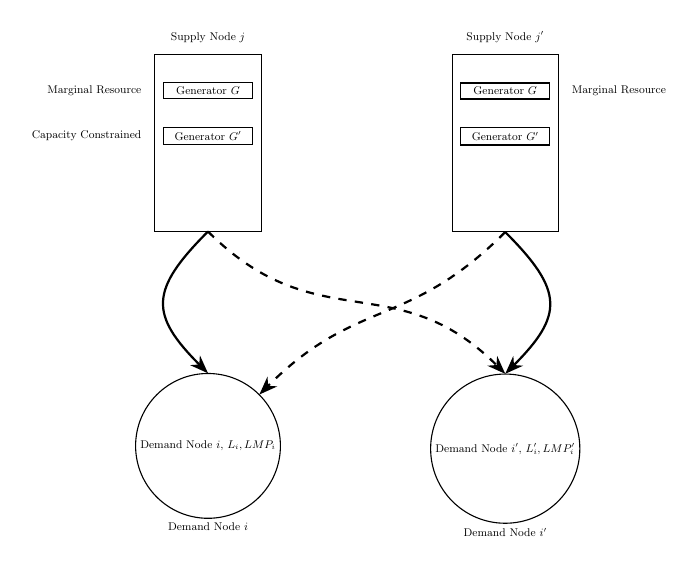
\begin{tikzpicture}[node distance=2cm, every node/.style={align=center, font=\small}, scale=.45, transform shape]

    % Supply Nodes with Labels above the boxes
    \node (supply1_label) [above=0.2cm] at (0,0) {Supply Node $j$};
    \node (supply1) [draw, rectangle, minimum width=3cm, minimum height=5cm, below=0.2cm of supply1_label] {};

    \node (supply2_label) [above=0.2cm, right=6cm of supply1_label] {Supply Node $j'$};
    \node (supply2) [draw, rectangle, minimum width=3cm, minimum height=5cm, below=0.2cm of supply2_label] {};

    % Generators at Supply Node j
    \node (gen1) [draw, rectangle, below=0.8cm of supply1.north, minimum width=2.5cm] {Generator $G$};
    \node (gen1_label) [left=0.5cm of gen1] {Marginal Resource};

    \node (gen2) [draw, rectangle, below=0.8cm of gen1, minimum width=2.5cm] {Generator $G'$};
    \node (gen2_label) [left=0.5cm of gen2] {Capacity Constrained};

    % Generators at Supply Node j'
    \node (gen3) [draw, rectangle, below=0.8cm of supply2.north, minimum width=2.5cm] {Generator $G$};
    \node (gen3_label) [right=0.5cm of gen3] {Marginal Resource};

    \node (gen4) [draw, rectangle, below=0.8cm of gen3, minimum width=2.5cm] {Generator $G'$};
    \node (gen4_label) [right=0.5cm of gen4] {};

    % Demand Nodes
    \node (demand1) [draw, circle, minimum width=1cm, below=4cm of supply1, label=below:{Demand Node $i$}] {Demand Node $i$, $L_i,LMP_i$};
    \node (demand2) [draw, circle, minimum width=1cm, below=4cm of supply2, label=below:{Demand Node $i'$}] {Demand Node $i'$, $L_i',LMP_i'$};

    % Arrows from Supply Nodes to Demand Nodes with Labels
    \draw[-{Stealth}, thick] (supply1.south) to [out=-135, in=135, looseness=1.5] (demand1.north) node[midway, left, xshift=-0.3cm] {};
    \draw[-{Stealth}, thick, dashed] (supply1.south) to [out=-45, in=135, looseness=1.2] (demand2.north) node[midway, above, xshift=0.5cm] {};
    \draw[-{Stealth}, thick, dashed] (supply2.south) to [out=-135, in=45, looseness=1.2] (demand1.north east) node[midway, right, xshift=-0.3cm] {};
    \draw[-{Stealth}, thick] (supply2.south) to [out=-45, in=45, looseness=1.5] (demand2.north) node[midway, right, xshift=-0.3cm] {};

\end{tikzpicture}
    \caption{Sample two-node network.}
    \label{SampleNetwork}
\end{figure}
\end{center}

\begin{center}
   \begin{figure}
    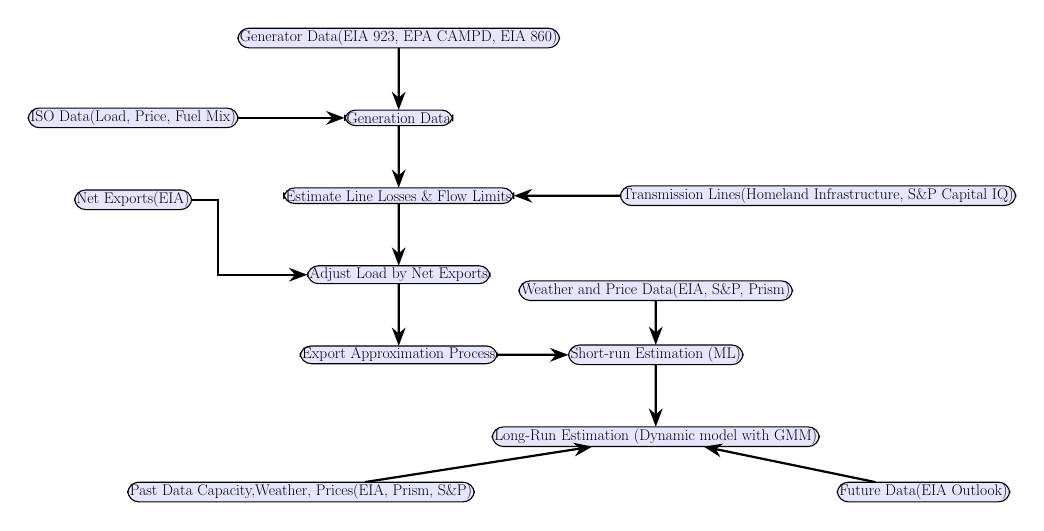
\begin{tikzpicture}[scale=0.225, every node/.style={transform shape},
        block/.style={rectangle, draw, text centered, rounded corners, minimum height=2.5em, minimum width=11em, fill=blue!10, font=\Huge},
        arrow/.style={-{Stealth[scale=1]}, thick},
        node distance=3cm  % Increase node distance for more space
    ]
        % Input Sources
        \node[block] (iso) {ISO Data \\ (Load, Price, Fuel Mix)};
        \node[block, below=of iso, yshift=-0.5cm] (net_exports) {Net Exports \\ (EIA)};

        % Generation Data and Generator Data
        \node[block, right=6cm of iso] (generation) {Generation Data};
        \node[block, above=of generation, yshift=0.5cm] (generator) {Generator Data \\ (EIA 923, EPA CAMPD, EIA 860)};

        % Processes
        \node[block, below=3.5cm of generation] (line_loss) {Estimate Line Losses \& Flow Limits};
        \node[block, below=of line_loss, yshift=-0.5cm] (load_adjust) {Adjust Load by Net Exports};

        % Export Estimation and Final Estimation
        \node[block, below=of load_adjust, yshift=-0.5cm] (exports) {Export Approximation Process};
        \node[block, right=4cm of exports] (estimation) {Short-run Estimation (ML)};
        
        % Long-Run Estimation and Inputs
        \node[block, below=of estimation, yshift=-0.5cm] (long_run) {Long-Run Estimation (Dynamic model with GMM)};
        \node[block, below left=2cm and 1cm of long_run] (past_data) {Past Data Capacity, \\ Weather, Prices \\ (EIA, Prism, S\&P)};
        \node[block, below right=2cm and 1cm of long_run] (future_data) {Future Data \\ (EIA Outlook)};
        
        % Additional Input: Weather and Price Data
        \node[block, above=of estimation, yshift=-0.5cm] (weather) {Weather and Price Data \\ (EIA, S\&P, Prism)};

        % Move Transmission Lines to the right of line_loss
        \node[block, right=6cm of line_loss] (transmission) {Transmission Lines \\ (Homeland Infrastructure, S\&P Capital IQ)};

        % Adjusted Arrows
        \draw[arrow] (iso.east) -- ++(1,0) |- (generation.west);  % ISO Data to Generation Data
        \draw[arrow] (generator) -- (generation);  % Generator Data directly above Generation Data
        \draw[arrow] (transmission.west) -- (line_loss.east);  % Transmission Lines to Estimate Line Losses
        \draw[arrow] (generation) -- (line_loss);  % Generation Data to Estimate Line Losses
        \draw[arrow] (net_exports.east) -| ++(1.5,0) |- (load_adjust.west);  % Net Exports to Adjust Load by Net Exports
        \draw[arrow] (line_loss) -- (load_adjust);  % Line Losses to Adjust Load by Net Exports
        \draw[arrow] (load_adjust) -- (exports);  % Adjust Load to Export Approximation Process
        \draw[arrow] (exports) -- (estimation);  % Export Process to Short-run Estimation
        \draw[arrow] (weather) -- (estimation);  % Weather and Price Data to Short-run Estimation
        \draw[arrow] (estimation) -- (long_run);  % Short-run Estimation to Long-run Estimation
        \draw[arrow] (past_data) -- (long_run);  % Past Data to Long-run Estimation
        \draw[arrow] (future_data) -- (long_run);  % Future Data to Long-run Estimation

    \end{tikzpicture}
    \caption{Dataset Construction Diagram.}
    \label{DataSetCreation}
    \end{figure}
\end{center}

\begin{figure}
    \centering
    
\includegraphics[width=0.5\linewidth]{images/PriceMap (2).png}
    \caption{Locational Marginal Price by Zone in Data.}
    \label{fig:PriceMap}
\end{figure}

\begin{figure}
    \centering
    
\includegraphics[width=0.5\linewidth]{images/GenerationCapacitySolarWind (1).png}
    \caption{Estimated Capacity Factor for Solar and Wind by ISO.}
    \label{fig:CapacityFactorbyISO}
\end{figure}

\begin{figure}
    \centering
    
\includegraphics[width=0.5\linewidth]{images/PriceLoadbyHour.png}
    \caption{Price and Load by Hour for entire dataset.}
    \label{fig:PriceLoad}
\end{figure}

\begin{figure}
    \centering
    
\includegraphics[width=0.5\linewidth]{images/ExportGraph (1).png}
    \caption{Map of Exports between Zones in the Model.}
    \label{ExportGraph}
\end{figure}


%\begin{figure}[hp]
%  \centering
%  \includegraphics[width=.6\textwidth]{../fig/placeholder.pdf}
%  \caption{Placeholder}
%  \label{fig:placeholder}
%\end{figure}




\clearpage

\appendix

\section{Operations Model Solution} \label{sec:appendixa}
\addcontentsline{toc}{section}{Appendix A: Operations Model Solution}

[PLACEHOLDER: Insert your operations model solution walkthrough here. This appendix should detail the algorithm for solving the short-run dispatch problem as a linear program, including the derivation of shadow prices for transmission constraints.]

\section{Long-run Model Computational Details} \label{sec:appendixb}
\addcontentsline{toc}{section}{Appendix B: Long-run Model Computational Details}

This appendix provides additional details on the computation of the long-run dynamic game equilibrium.

\subsection{State Space Discretization}

[PLACEHOLDER: Provide additional justification for discretization choices and sensitivity analysis if available.]

\subsection{Convergence Criteria}

[PLACEHOLDER: Detail the convergence criteria used in the nested fixed point algorithm.]

\subsection{Computational Performance}

[PLACEHOLDER: Report computation times and any parallelization strategies employed.]

\section{Transmission Capacity and Line Loss Estimation} \label{sec:appendixc}
\addcontentsline{toc}{section}{Appendix C: Transmission Capacity and Line Loss Estimation}

This appendix details the engineering assumptions used to estimate transmission capacity and line losses from the HIFLD data following \cite{arkolakis2023clean}.

[PLACEHOLDER: Insert technical details on line loss and capacity estimation methodology.]

\section{Additional Robustness Checks} \label{sec:appendixd}
\addcontentsline{toc}{section}{Appendix D: Additional Robustness Checks}

[PLACEHOLDER: Include any robustness checks such as alternative discretizations, different moment conditions, or sensitivity to key assumptions.]



\end{document}
